\newpage

\section{Modulationsverfahren}

Das Verfahren, um binäre Daten auf ein analoges Trägersignal zu bringen, wird als digitale Modulation bezeichnet. 
In Abbildung \ref{fig:ook_modulation} sind die Modulationsverfahren ASK und FSK dargestellt. ASK steht für \textit{Amplitude Shift Keying} und FSK für \textit{Frequency Shift Keying}. 
Im ersten Graphen von oben ist das digitale Signal dargestellt, das moduliert werden soll.
Im zweiten Gaphen ist das mit FSK modulierte Signal dargestellt. Der maximale Frequenzunterschied wird dabei als Frequenzhub $\Delta F$ bezeichnet.
Darunter ist das mit ASK modulierte Signal dargestellt. Es handelt sich dabei um sogenanntes \textit{On-Off-Keying} (OOK), bei dem das Signal entweder an oder aus ist.

\begin{aufgabe}
    Bestimmen Sie für Abbildung \ref{fig:ook_modulation} die Trägerfrequenz und den Frequenzhub $\Delta F$ des FSK-Signals.
\end{aufgabe}
\karierteBox{5}

\begin{lösung}
    Durch Ablesen im Graphen bestimmen:

    \[
    f_{0} = \frac{2}{\SI{0,2}{\milli\second}} = \SI{10}{\kilo\hertz}
    \]

    \[
    f_{1} = \frac{3}{\SI{0,2}{\milli\second}} = \SI{15}{\kilo\hertz}
    \]

    \[
    \Delta F = f_{1} - f_{0} = \SI{5}{\kilo\hertz}
    \]
\end{lösung}

\begin{figure}[H]
    \centering
    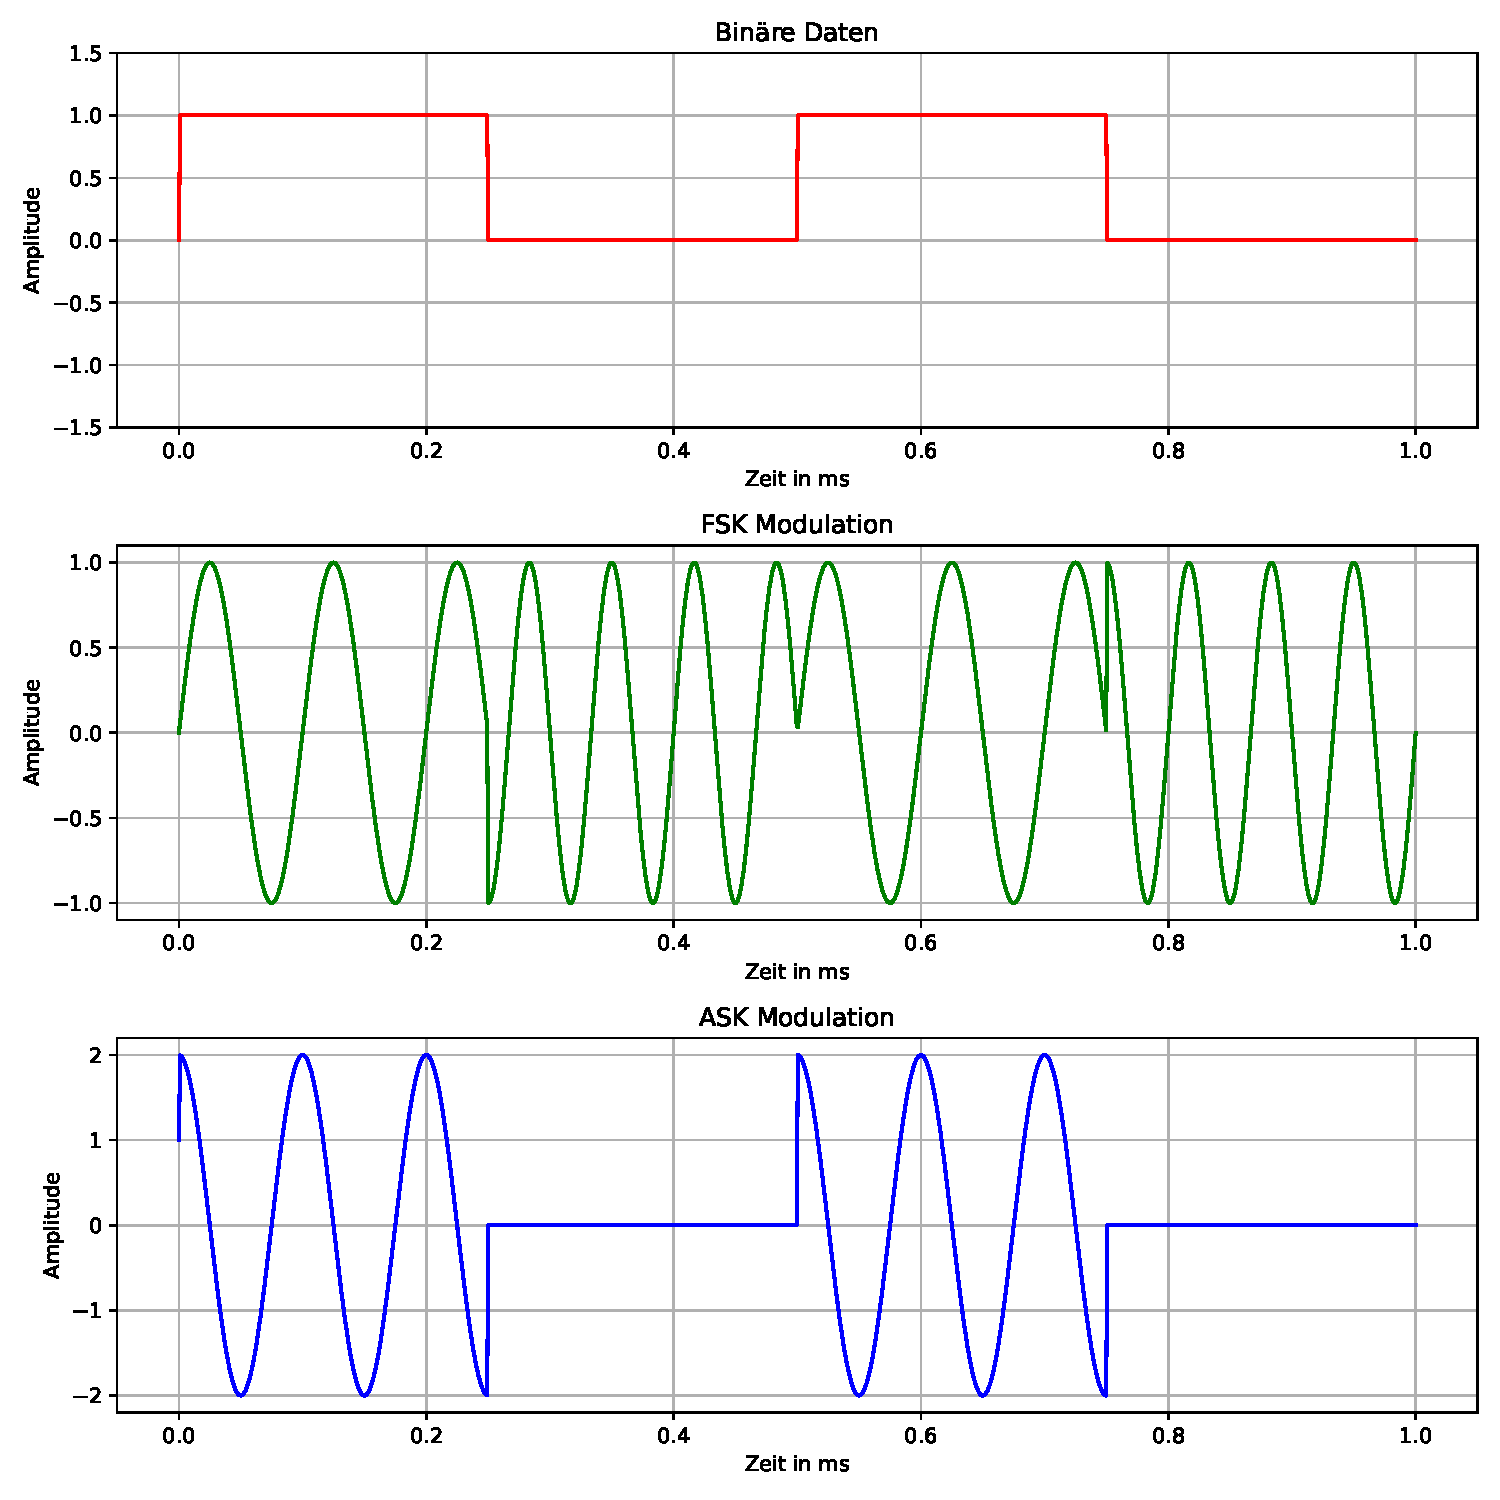
\includegraphics[width=0.8\textwidth]{images/ASK_FSK.pdf}
    \caption{Modulationsverfahren: ASK und FSK.}
    \label{fig:ook_modulation}
\end{figure}

\section{Antennen und Wellenlängen}

Eine Annäherung für eine Stabantenne ist der Hertzsche Dipol. Das Strahlungsmuster, dass sich für den hertzschen Dipol ergibt, ist in Abbildung \ref{3d_pattern} in 3D und in Abbildung \ref{2d_pattern} in 2D für die drei Hauptebenen in kartesischen Koordinaten dargestellt.

\begin{figure}[H]
    \centering
    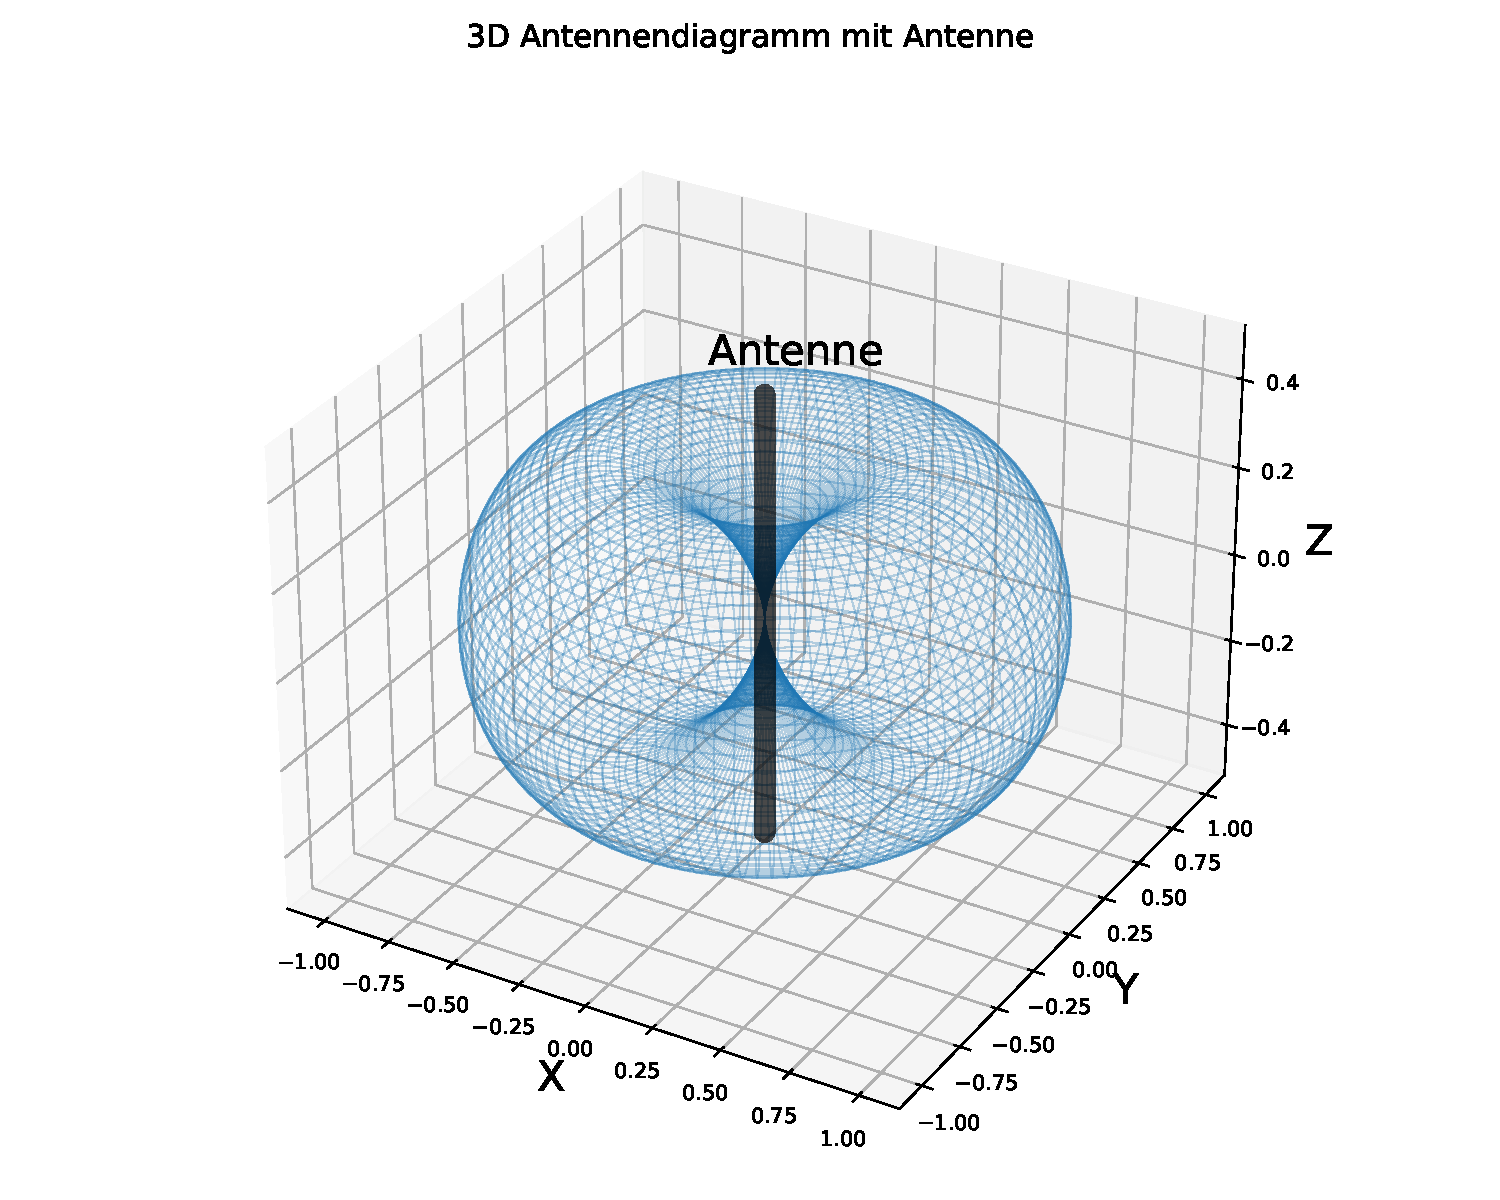
\includegraphics[width=0.8\textwidth]{images/3d_radiation_pattern.pdf}
    \caption{3D Strahlungsmuster des Hertzschen Dipols.}
    \label{3d_pattern}
\end{figure}

\begin{aufgabe}
Zeichnen Sie das Strahlungsmuster der Stabantenne in 2D in den drei Hauptebenen der kartesischen Koordinaten, die in Abbildung \ref{2d_pattern} dargestellt sind.
\end{aufgabe}
\begin{figure}[H]
    \centering
    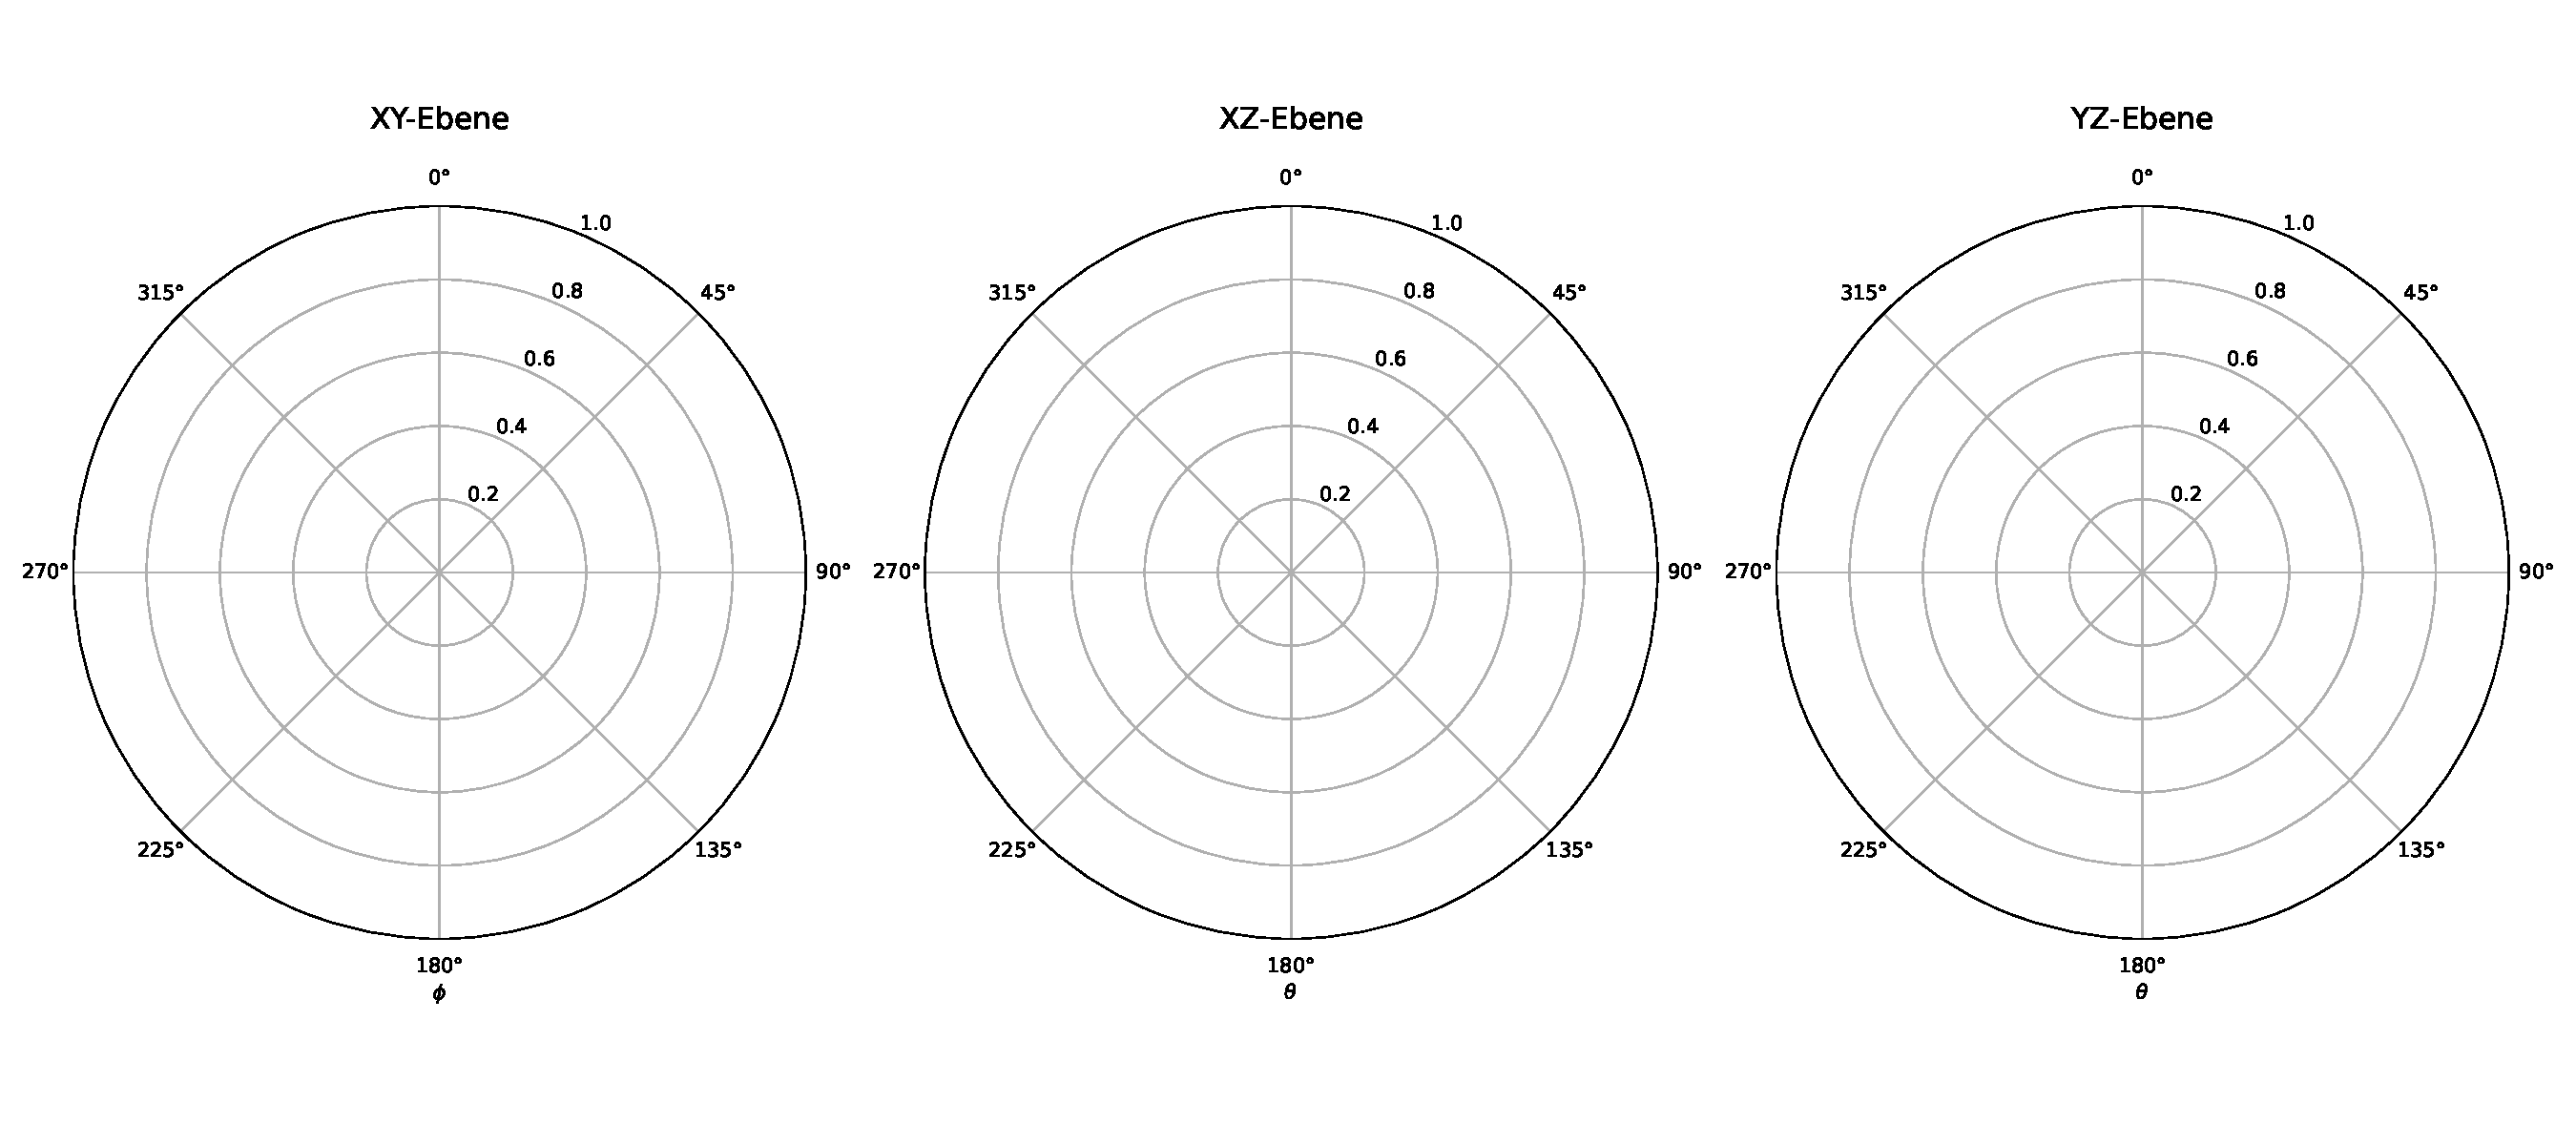
\includegraphics[width=.95\textwidth]{images/polar_radiation_pattern_empty.pdf}
    \caption{Hier soll das Strahlungsmuster der Stabantenne in 2D gezeichnet werden.}
    \label{2d_pattern}
\end{figure}

\begin{lösung}
    \centering
    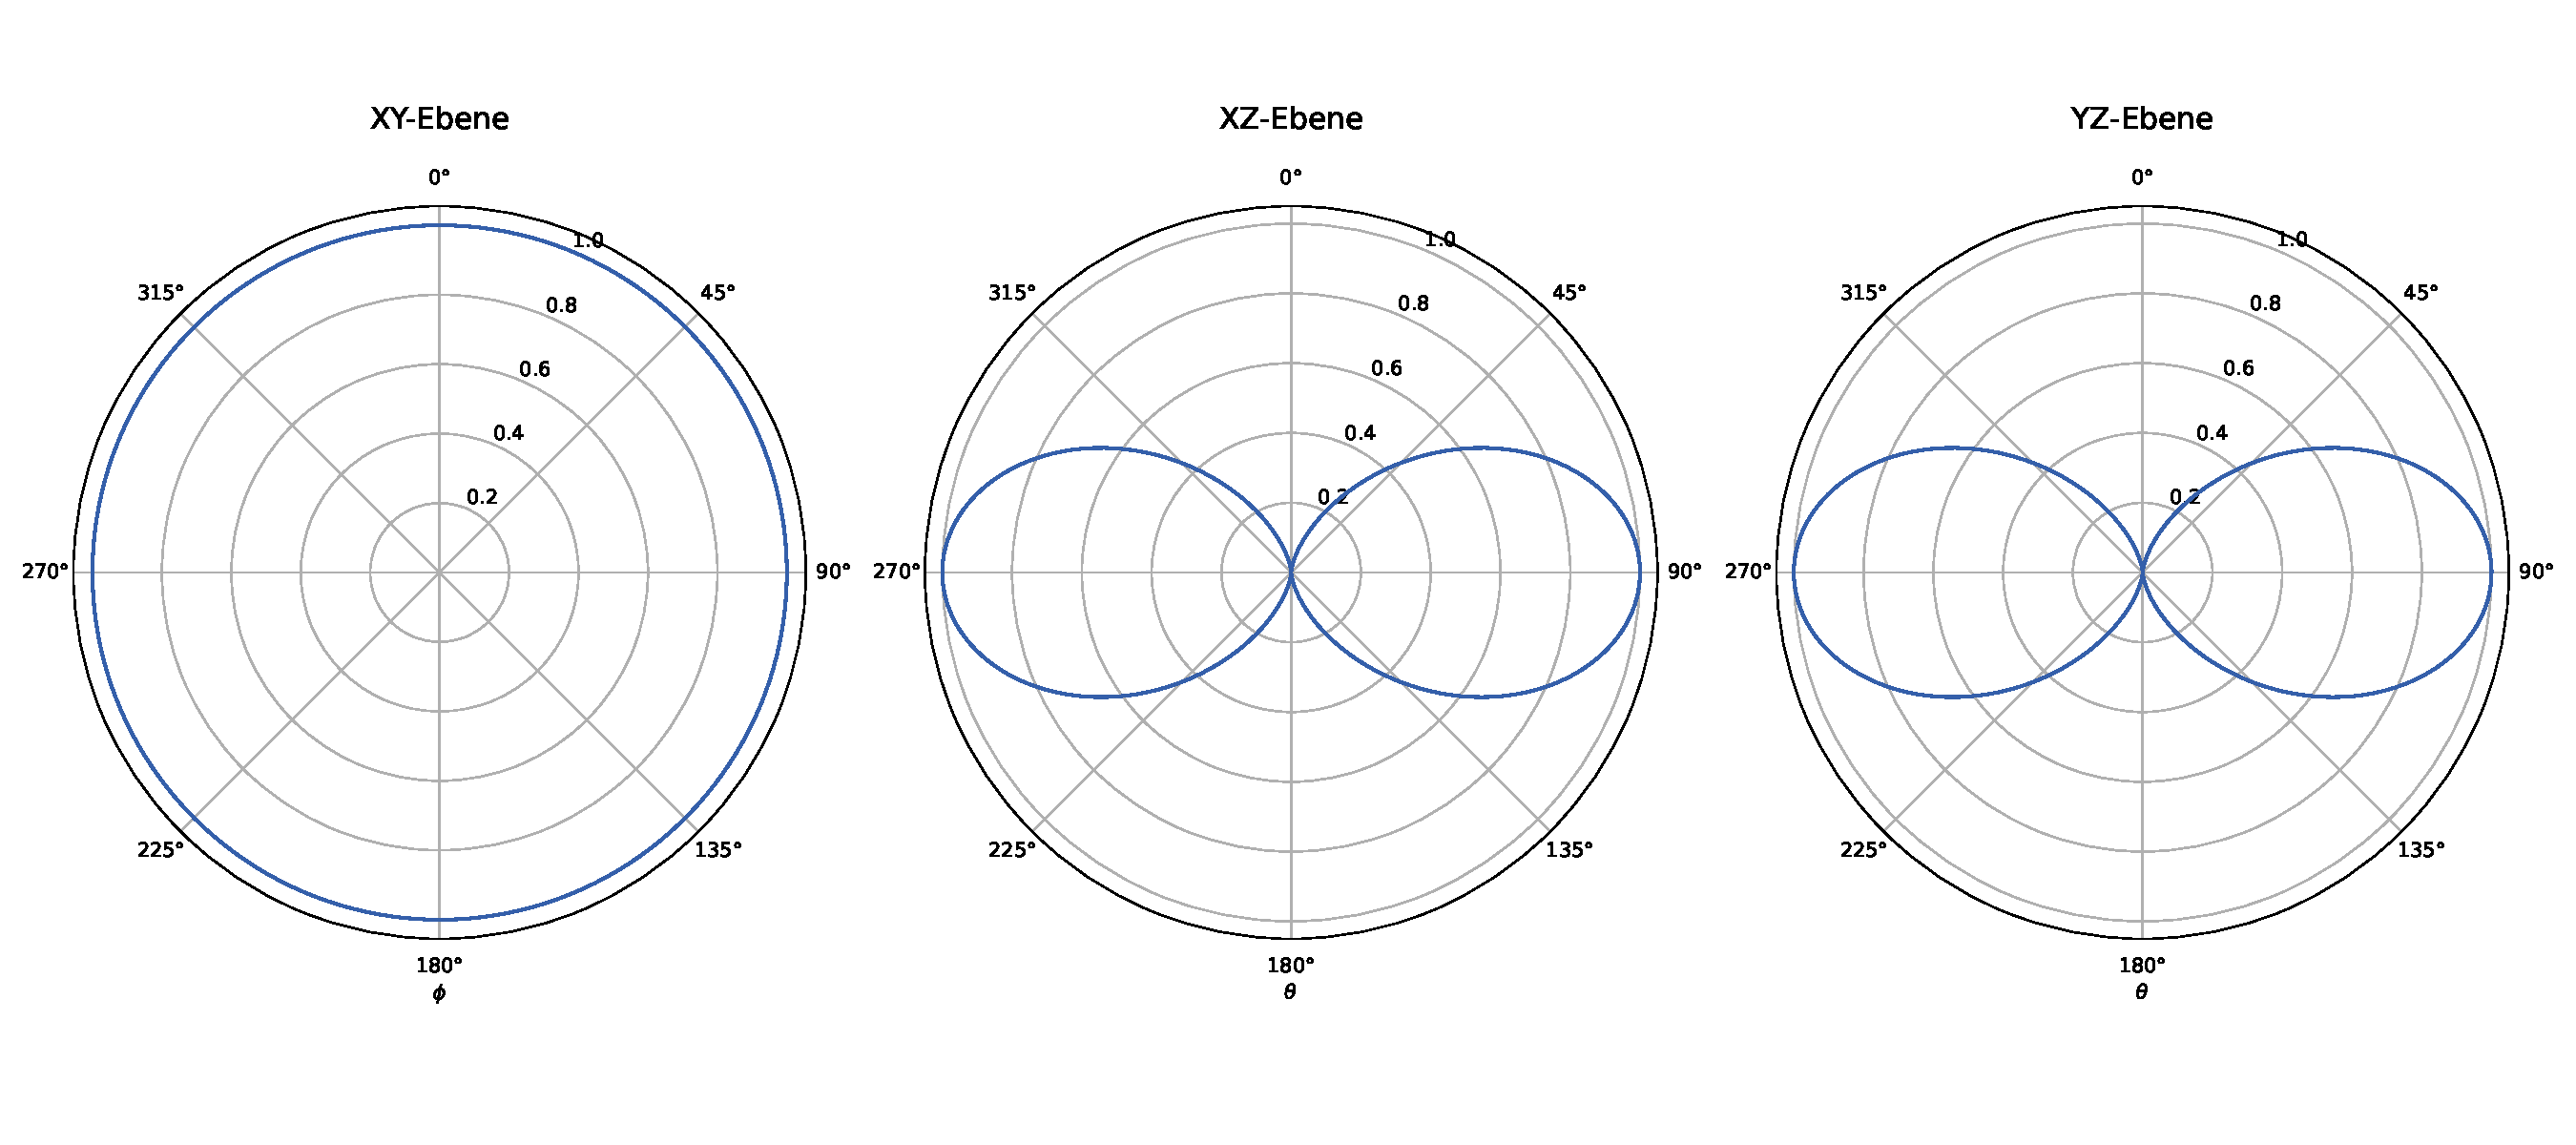
\includegraphics[width=.9\textwidth]{images/polar_radiation_pattern.pdf}
    \captionof{figure}{2D Strahlungsmuster des Hertzschen Dipols.}
\end{lösung}




\section{Arduino und Transmitter Anschlüsse}
In diesem Abschnitt werden die Anschlüsse von Transmitter und Arduino beschrieben. Sie sind in Tabelle \ref{tab:arduino_transmitter_connections} zusammengefasst.

\begin{table}[H]
\centering
\noindent
\begin{tabular}{l l}
    \toprule
    \multicolumn{2}{c}{\textbf{Arduino}} \\
    \midrule
    \texttt{GND} & Masse \\
    \texttt{VCC} & Versorgung (5V/3.3V) \\
    \texttt{Digital I/O} & Digitale Ein-/Ausgänge \\
    \texttt{Analog In} & Analoge Eingänge \\
    \addlinespace % Fügt eine Leerzeile für eine visuelle Trennung ein
    \addlinespace
    \multicolumn{2}{c}{\textbf{Transmitter}} \\
    \midrule
    \texttt{GND} & Masse \\
    \texttt{VCC} & Versorgung \\
    \texttt{DATA} & Daten-Eingang \\
    \texttt{ANT} & Antenne \\
    \bottomrule

\end{tabular}
\caption{Anschlüsse des Arduino und des Transmitters}
\label{tab:arduino_transmitter_connections}
\end{table}


\begin{aufgabe}
    Verdrahten Sie die Bauteile, die Sie an Ihrem Arbeitsplatz finden und in Abbildung \ref{fig:arduino_433_schematic_skript} gezeigt sind sinnvoll miteinander.
\end{aufgabe}


\begin{figure}[H]
\centering
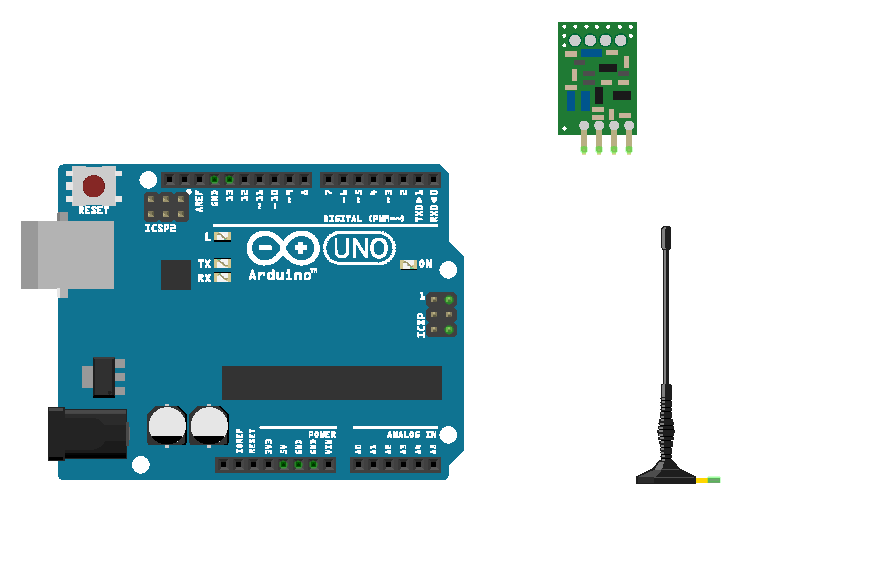
\includegraphics[width=0.8\textwidth]{images/Arduino_433_Sketch_Skript.pdf}
\caption{Schematic des Arduino mit Transmitter und Antenne.}
\label{fig:arduino_433_schematic_skript}
\end{figure}

\begin{lösung}

    \centering
    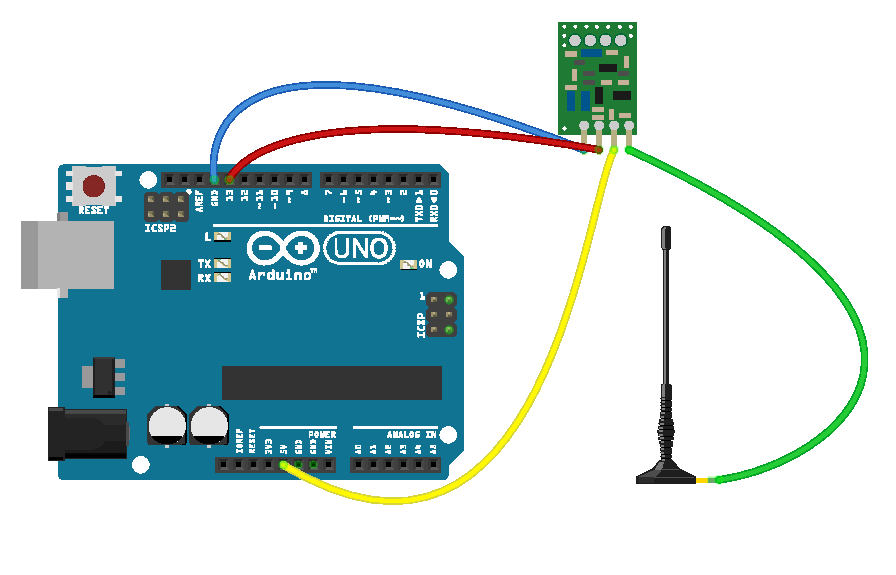
\includegraphics[width=0.8\textwidth]{images/Arduino_433_Sketch.pdf}
    \captionof{figure}{Schematic des Arduino mit $=\SI{433}{\mega\hertz}$ Transmitter, Antenne und korrekter Verdrahtung.}
\end{lösung}


\begin{aufgabe}
Ermitteln Sie auf dem RF-Transmitter die Trägerfrequenz. Entwerfen Sie eine Drahtantenne, die ein Viertel der Wellenlänge, also $\lambda/4$ lang ist. Verwenden Sie die Formel $\lambda = \frac{c}{f}$, wobei $c$ die Lichtgeschwindigkeit im Vakuum ($=\SI{3e8}{\meter\per\second}$) ist.
\end{aufgabe}
\karierteBox{5}

\begin{lösung}
Die Wellenlänge \(\lambda\) des Signals kann mit der Formel \(\lambda = \frac{c}{f}\) berechnet werden. Für \(f = 433\) MHz ergibt sich:

\[
\lambda = \frac{\SI{3e8}{\meter\per\second}}{\SI{433}{\mega\hertz}} \approx 0.693 \text{ m}
\]

Die Länge der Drahtantenne, die einem Viertel der Wellenlänge entspricht, ist daher:

\[
\frac{\lambda}{4} = \frac{0.693 \text{ m}}{4} \approx 0.173 \text{ m}
\]

Die Antenne sollte also etwa 17.3 cm lang sein.
\end{lösung}
